%%%%%%%%%%%%%%%%%%%%Tesis File%%%%%%%%%%%%%%%%%%%%%%%%%%%%%%%%%%%%%%%%%%%%%%%%%%%%%

\documentclass[12pt]{book}
\usepackage{cite}
\usepackage{amssymb}
\usepackage{amsthm}
\usepackage{amsmath}
\usepackage[pdftex]{graphicx}
\usepackage{setspace}
\usepackage{mathrsfs}
\usepackage{float}

%Theorems
\newtheorem{definition}{Definition}




%Commands

%Prior, posterior and likelihood
\newcommand{\post}{\mathbb{P}_{post}}
\newcommand{\like}{\mathbb{P}_{like}}
\newcommand{\prior}{\mathbb{P}_{prior}}
\newcommand{\p}{\mathbb{P}}


%Other commands
\newcommand{\E}{\mathbb{E}} %Expectation
\newcommand{\tvs}{\mathscr{X}} %TVS symbol







\begin{document}
\setlength{\unitlength}{1 cm} %Especificar unidad de trabajo
\thispagestyle{empty}
\begin{center}
    %\begin{picture}(18,4)
    %\centering
    
\includegraphics[scale=0.5]{log.png} \\[1cm]
    %\end{picture}
\textbf{{\LARGE Simon Fraser University}\\[0.5cm]
{\LARGE Faculty of Sciences, Math Department}}\\[1.25cm]
\begin{doublespace}
{\huge \textbf{Here comes the title}}\\[1.5cm]
\end{doublespace}
{\large Juan Gabriel Garc{\'i}a Osorio}\\[1cm]
Advisor: John Stockie\\[1cm]
Commitee: Paul Tupper\\[1cm]
Burnaby B.C - May  2017
\end{center}

\newpage
\tableofcontents


%%%%%%%%%%%%%%%%%%%%%%%%%%%%%%%%Chapter 0 %%%%%%%%%%%%%%%%%%%%%%%%%%%%%%%%%%%%%%%%%%%%%%%%%%%%%%%
\chapter*{Acknowlegments}

\newpage


%%%%%%%%%%%%%%%%%%%%%%%%%%%%%%%Chapter 1: Introduction %%%%%%%%%%%%%%%%%%%%%%%%%%%%%%%%%%%%%%%%%%
\chapter{Introduction}

\newpage

%%%%%%%%%%%%%%%%%%%%%%%%%%%%%%Chapter 2: Theoretical and Computational Framework %%%%%%%%%%%%%%%%
\chapter{Theoretical and Computational Framework}
%\pdfmarkupcomment[markup=Squiggly,color=green]{what eve}{Change this shit}


The foundations of  our approach to estimate parameters and solve inverse problems is  the 
framework of Bayesian statistics. Unlike frequentist statistics, in the Bayesian approach, randomness
is a measure of uncertainty, is not a matter of frequency . For instance a question like
what is the probability of having  life in Mars? If the answer is say 0.01, in the frequentist
stastistics framework, this number is interpreted as, for every hundred times we go to 
mars under identical circumstances, one of those times we will find life there. In the Bayesian
approach the number 0.01 is interpreted as: given our current level of knowledge about mars
we think that is very unlikely that mars shelters life. Clearly there is a big phylosofical
difference between these two approaches that has a direct impact in how far reaching is each point of view  \cite{jaynes2003probability}.


%Talking about Bayes rule
In real life the uncertainty associated to a  measurement or  quantity of interest is usually 
connected  with the uncertainty  of other variables involved in the problem under study. 
At this point we mention that When we talk about uncertainty we are talking about every possible 
source of randomness  or  lack of information. That is, the use of the word uncertainty in this work
is related to either epistemic (A phenomenon might not be random but the complete lack of 
understanding of it makes us see it as random) or aleatory (Inherent to the nature of phenomenon, for 
example this is the kind of randomness physicists believe is happening in quantum mechanics)
\cite{kennedy2001bayesian}.
In general the connection between the different variables is far from trivial and hard to assess.
Bayesian methodology provides a rigurous framework for the study of 
this connection, using whatever information
is available for the problem. The cornerstone of this idea
in the mathematical language is the  Bayes formula 
\begin{equation}\label{eqnBayes}
\post(A|B)=\frac{\like(B|A)\prior(A)}{\p(B)}.
\end{equation}

To explain in detail the above equation, let us first do the following defintion
\cite{dudley2002real}
\begin{definition}\label{dfn:probabilitytriple}
A probability space is a triple $(\Omega,\mathscr{F},\p)$, where $\Omega$ is a set called 
sample space.
The element $\mathscr{F}$ is a subset of the power set of $\Omega$ that satisfies
\begin{enumerate}
\item $\emptyset,\Omega\in\mathscr{F}$.
\item If $A\in\mathscr{F}$ then $A^{c}\in\mathscr{F}$.
\item If $A_{1},A_{2},\ldots \in\mathscr{F}$ then $\bigcup_{i\in\mathbb{N}}A_{i}\in\mathscr{F}$.
\end{enumerate}
A set that satisfies properties 1 to 3 is called a $\sigma-$ algebra and its elements are called
events. The map $\p:\mathscr{F}\rightarrow [0,1]$ satisfies
\begin{enumerate}
\item $\p(\Omega)=1$.
\item If $A_{1},A_{2},\ldots \in\mathscr{F}$ are pairwise disjoint, then 
\begin{equation*}
\p(\bigcup_{i\in\mathbb{N}}A_{i})=\sum_{i\in\mathbb{N}}\p(A_{i}).
\end{equation*}
\end{enumerate}
$\p$ is called a probability measure.
\end{definition}


In equation (\ref{eqnBayes}), $\p,\prior,\like,\post$ are different probability measures defined in the
same sample space $\Omega$. The sets $A$ and $B$ are subsets of the sample space $\Omega$ and 
are elements of the associated $\sigma-$algebra $\mathscr{F}$. The bar in the probability
measures e.g. $\like(\cdot|\cdot)$, means conditional probability. Let us introduce some terminology:
 the term $\like(B|A)$ is called the \textit{likelihood} of $B$ given $A$, $\prior(A)$ is called the 
\textit{prior} for $A$. The prior expreses how much we believe the event $A$ to happen without assuming
anything about how the event $B$ might influence the event $A$. 
The term $\p(B)$ is a \textit{normalization constant} defined as 
\begin{equation*}
Z(B)=\int_{\Omega} \like(B|A)\prior(A)d\p.
\end{equation*}
The term $\post(A|B)$ is  the \textit{posterior}. The posterior contains all the information 
gained when comparing our beliefs (prior) with experimental data (likelihood). The posterior
is the \textit{solution of an inverse problem} when using the  Bayesian framework.

Simply put  formula (\ref{eqnBayes}) implies: the probability that the event $A$ given that
the event $B$ has already occurred is proportional to the probability of the event $B$ given
that the event $A$ has already happened weighted by the prior probability of $A$.
\newline



%Ilustratory example
This interpretation of Bayes rule serves as a motivation for using it in the field of inverse problems. 
Inverse problems are  of the type `find the cause of this effect'. This name is relative to what is known
as the direct problem. These are problems of the type `find the effect of this cause'. Often inverse problems
 ill-posed, this means
that these problems might  not satisfy one or more of the following properties \cite{lebedev2012functional}:
\begin{itemize}
\item Existence: There exists a solution for the problem.
\item Uniqueness: The problem has a unique solution.
\item Stability: Small changes in inputs result in small changes in outputs.
\end{itemize}
This is a serious issue. If the problem under study has at least one solution but  is not stable, for example, 
how can we assess the accuracy of the result obtained? An statistical approach is called for under
this setting. But the most important reason of why the Bayesian framework is useful to solve inverse problems
is that Bayes rule unifies the problem of 'find the cause of this effect' (e.g. finding the posterior)
with the direct problem of `find the effect of this cause' (e.g. finding the likelihood).

Let us be precise of how the Bayesian approach can be used to solve inverse problems with an example. 
Consider the problem of finding the location where a rock that smashed a window was thrown. We can
start by considering the following events
\begin{center}
$A$=x,y,z coordinates where the rock was thrown.\newline
$B$=x,y,z coordinates where the rock hit the window.
\end{center}
In this case Bayes formula  tells us that if we want to estimate the likely locations  where the rock was 
thrown from (find the posterior probability), given that we 
know the coordinates where it hit the window we need to include our prior believe on where
do we think the rock was actually thrown (Setting a prior probability). Also it is necessary
to find the connection with the direct problem. In this case the direct problem is to find where
the rock hit the window assuming that we know where it was thrown (find the likelihood probability) 
\newline



Let us evaluate how we could estimate the different probabilities mentioned in the previous paragraph. 
First, to find the likelihood
we need to know how the rock's impact position  in the window  is related to the launch location 
. If we treat air resistance as a source of uncertainty  we can use
the kinematics equations  for parabolic trajectories to get \cite{arnol2013mathematical}
\begin{equation}\label{eqnKinematics}
\textbf{r}=\textbf{r}_{0}+\textbf{v}_{0}t+\frac{1}{2}\textbf{g}t^{2},
\end{equation} 
where $\textbf{r}$ and $\textbf{r}_{0}$ are the final and initial position of the rock respectively, 
$\textbf{v}_{0}$ is 
the initial velocity  and $\textbf{g}$ is the gravity vector. The scalar $t$ represents time.
In a more physical language, to estimate the likelihood it is necessary to estimate $\textbf{r}$ (where the 
rock hit the window) assuming we know $\textbf{r}_{0}$ (where it was thrown). 
To do so,
we  need to estimate the initial velocity of the rock $\textbf{v}_{0}$. 
Once all the other variables are identified the value of $t$ can be computed in a straightforward manner. 

Equations in physics are just models of reality and as such are just an approximation to it. To take
this into account we add an extra layer to the model by adding a random parameter that accounts
for the discrepancy of our model. We propose 
\begin{equation*}
\textbf{r}=\textbf{r}_{0}+\textbf{v}_{0}t+\frac{1}{2}\textbf{g}t^{2}+\mathbf{\epsilon},
\end{equation*} 
where $\mathbf{\epsilon}$ is a random vector distributed as $\vec{\epsilon}\sim\mathscr{N}(0,\sigma I)$. Here $I$
represents the $3\times 3$ identity matrix and $\sigma>0$ parametrizes one belief in quantifing the 
accuracy  
of equation (\ref{eqnKinematics}).  By introducing a random variable into the model
we can now think of all of the variables involved  in equation (\ref{eqnKinematics})
as random, that is, we now look at the  associated stochastic equation. With this notation
we can cast equation (\ref{eqnBayes}) into  (assuming independence between $\textbf{r}_{0}$ and $\textbf{v}_{0}$)
\begin{equation}\label{eqnpostrock}
\post(\textbf{r}_{0}|\textbf{r},\textbf{v}_{0})=\frac{\like(\textbf{r}|\textbf{r}_{0},\textbf{v}_{0})
\prior(\textbf{r}_{0})}{\p(\textbf{r}|\textbf{v}_{0})}.
\end{equation}



Since $\mathbf{\epsilon}$ is Gaussian we can readily obtain \cite{Somersalo}
\begin{equation*}
\textbf{r}|\textbf{r}_{0},\textbf{v}_{0}\sim \mathscr{N}(\textbf{r}_{0}+\textbf{v}_{0}t+\frac{1}{2}\textbf{g}t^{2}
,\sigma I).
\end{equation*}

This equation gives an explicit density for the likelihood. We now turn our attention to model the prior.
Suppose that we suspect that the rock was thrown from the bedroom of one of our neighboors.
 One way to model this suspicion is to assume a prior distribution on $\textbf{r}_{0}$ as
\begin{equation*}
\textbf{r}_{0}\sim\mathscr{N}(\textbf{z},\lambda I),
\end{equation*}
where $\textbf{z}$ is the coordinate vector of the center of mass of neighbohr's room and $\lambda$ represents 
the variance of the launch location around the point $\textbf{z}$. We note that  this is one way to model 
 prior knowledge and other priors are also possible for our problem.

The last quantity to find is   the normalization constant $\p(\textbf{r}|\textbf{v}_{0})$. Since all
probabilities are normalized we get
\begin{eqnarray*}
1=\int_{\mathbb{R}^{3}}\post(\textbf{r}_{0}|\textbf{r},\textbf{v}_{0})d\textbf{r}_{0}\\
=\int_{\mathbb{R}^{3}}\frac{\like(\textbf{r}|\textbf{r}_{0},\textbf{v}_{0})
\prior(\textbf{r}_{0})}{\p(\textbf{r}|\textbf{v}_{0})}d\textbf{r}_{0}.
\end{eqnarray*} 
Since the denominator in the last integrand is a constant with respect to the variable of integration 
we conclude
\begin{equation*}
\p(\textbf{r}|\textbf{v}_{0})=\int_{\mathbb{R}^{3}}\like(\textbf{r}|\textbf{r}_{0},\textbf{v}_{0})
\prior(\textbf{r}_{0})d\textbf{r}_{0}.
\end{equation*}


Having the likelihood, prior and normalization constant allow us to compute the posterior using
Bayes rule. Note that the posterior is a probability density so in order to obtain useful
statistics,  is necessary to sample from it. How to sample from a probability density is going
to be explained in the next chapter. For the moment assume we have the means to sample from the 
posterior in equation (\ref{eqnpostrock}). Having samples from the posterior we can obtain
pointwise estimates of the parameters of interest. Common choices of pointwise estimates
include
\begin{eqnarray*}
\textbf{r}_{MAP}=argmax_{\textbf{r}_{0}}\post(\textbf{r}_{0}|\textbf{r},\textbf{v}_{0}). 
\qquad\text{(Maximum a posteriori)}\\
\textbf{r}_{CM}=\int_{\mathbb{R}^{3}}\textbf{r}_{0}\post(\textbf{r}_{0}|\textbf{r},\textbf{v}_{0})d\textbf{r}_{0}.
\qquad\text{(Conditional mean)}. \\
\textbf{r}_{ML}=argmax_{\textbf{r}_{0}}\post(\textbf{r}_{0}|\textbf{r},\textbf{v}_{0}).
\qquad\text{(Maximum likelihood)}
\end{eqnarray*}

Each  of these estimates have strenghts and weaknesess. If the posterior is bimodal, then the conditional
mean might point at a value with very low probability, whereas the maximum a posteriori might be more 
relaible. If the posterior has no critical points then the mean might be use as a point estimate. We can 
also assess how confident we are about the point estimate. If $\textbf{r}^{*}$ is our point
estimate we can calculate $\alpha>0$ such that
\begin{equation*}
\int_{B(\textbf{r}^{*},\alpha)}\post(\textbf{r}_{0}|\textbf{r},\textbf{v}_{0})d\textbf{r}_{0}=0.95,
\end{equation*}
where $B(\textbf{r}^{*},\alpha)$ is a ball centered at $\textbf{r}_{0}$ and radius $\alpha$. This 
uncertainty estimate can be think of as a generalization of a Bayesian $95\%$ confidence interval.
Another way to estimate uncertainty is by calculating the variance of $\textbf{r}$ with respect
to the measure $\post$. 
\newline

We solved our mistery, we have a way to estimate where the rock was thrown and a way to measure how
confident we are about this estimate. 
\newline


%Caveats of computing complex models
Practial problems are often substantially more challenging than the above example. Often times we have to 
deal with several issues such as 

\begin{enumerate}
\item Uncertainties in experimental measurements.
\item Lack of sufficient information and data.
\item Computational complexity of  physical models that are too expensive to evaluate.
\item Parameters of interest belong to high dimensional spaces so the associated probability density is 
hard to sample from.
\item Evaluating any of the possible point estimates for the quantity of interest might be very hard.
\end{enumerate}
In the problem described in the Chapter 1, we have to deal with the above mentioned issues.
In this chapter we are going to discuss our approach to deal with issues 3, 4 and 5 above. We 
ommit 1 and 2, since these issues are intrinsic in the physics of the problem and   the methodology used 
to obtain the experimental data, both of these aspects are out of our hands.


%%%%Dealing with computational complexity
\section{Dealing with  the computational complexity of the physical model}
Models of physical processes are often complex and are  expensive to simulate numerically.
Following O'Hagan  \cite{o2006bayesian}, we think of our  mathematical model as a function
$M(\cdot)$ that takes a vector $\textbf{x}$ of inputs and gives back a vector $\textbf{y}$ of outputs.  
Mathematical models are approximations to explain the reality and as such there is uncertainty associated
to them. Since mathematical models are expensive,
this means that estimating the uncertainty via   classical methods such  as in 
\cite{saltelli2000sensitivity} is not feasible. Here the concept of emulator as defined in \cite{o2006bayesian} 
comes into play. We 
approximate the function $M(\cdot)$, which is assumed to be expensive to evaluate,
 with a function $\hat{M}(\cdot)$, that is cheaper to evaluate. To construct an approximation,   
we  associate a 
probability distribution to each value $M(x)$ and then take the mean
of this distribution as $\hat{M}(x)$, for example. We will call such approximation $\hat{M}(\cdot)$ and emulator. 
Following \cite{o2006bayesian} we create the emulator in the following steps 
\begin{itemize}
\item At points $\textbf{x}$  were we know the output of the mathematical model i.e. $M(\textbf{x})$,
the emulator shoudl satisfy $\hat{M}(\textbf{x})=M(\textbf{x})$.
\item For the points $\textbf{x}^{*}$ where we don't know the output $M(\textbf{x}^{*})$, the emulator should
give back an estimate $\hat{M}(\textbf{x}^{*})$, based on the distribution for $M(\textbf{x}^{*})$. 
That estimate should reflect the uncertainty associated with
the interpolation/extrapolation done at that point.
\end{itemize} 


%Talking about Gaussian processes

A very popular  method to produce an emulator with the desired
extrapolation/interpolation properties is what is known as a  Gaussian process (GP).  

\subsection{Gaussian Processes}

\begin{definition}\label{dfnGP}
A GP is a collection of random variables $\{f(x)\}_{x\in X}$, for some index family $X$,
 such that any finite set of them has a jointly
Gaussian distribution \cite{rasmussen2006gaussian}. 
\end{definition}

A GP is specified by two quantities, the mean function and the covariance function. 
Following the same notation as in Rasmussen \cite{rasmussen2006gaussian} we set
\begin{eqnarray*}
m(x)=\E(f(x)),\\
k(x,x')=\E((f(x)-m(x))(f(x')-m(x'))).
\end{eqnarray*}
So if $\{f(x)\}$ is a GP with mean $m(x)$ and covariance $k(x,x')$ we will write
\begin{equation*}
f(x)\sim \textbf{GP}(m(x),k(x,x')).
\end{equation*} 

To understand the notion of a GP observe that what  
we are trying to do is to approximate a function $f(\cdot)$, then
the symbol $f(x)$ represents a random variable whose realizations are  the possible values of the
 function $f(\cdot)$ at $x$ and $m(x)$ is the best approximation we can do to predict the actual value 
of $f(\cdot)$ at that point $x$. The uncertainty associated to that prediction is going to be related
to the quantity $k(x,x)$.

Since we are going to use GP to fit  data in a high dimensional euclidean space, it will be convenient to think
of the set of index $X$ in definition \ref{dfnGP} as $\mathbb{R}^{n}$ for some $n\geq 1$. 
\newline

The reason why the definition of a Gaussian process is useful and powerful is because a GP is 
completely characterized by $m(x)$ and $k(x,x')$\footnote{ $k(x,x')$ 
is usually known as the kernel of the GP}\cite{lifshits2012lectures}. Therefore to fit and 
predict using GPs we only need to define just two quantities. For example the way to choose
the covariance kernel is with the aid of some real valued function. For example a very common covariance
function is given by what is called the squared exponential (SE)
\begin{equation}\label{eqnsquareexponential}
k(x,x')=e^{-\frac{1}{2}\|x-x'\|_{2}^{2}}.
\end{equation}
In this case this definition of the covariance is telling us that points that are close to each other
are highly correlated whereas far away points has a correlation that decays exponentially fast with distance.
There are some `standard' ways to choose the covariance function depending on the kind
of regularity we want for the GP fitting. To see what is the relation between regularity
of the fitting and the kernel we need to realize that once the covariance function has been 
specified we end up with a distributions over some function space. Talking 
about distribution over spaces of functions is a delicate topic that has to be done in a rigorous manner.
That is why at this point it is convenient to digress for a moment an talk about distributions in 
function spaces. The details presented here follow from \cite{lifshits2012lectures}.

\subsubsection{Distributions Over Function Spaces}
Since in general the relevant function spaces (e.g. $L^{p}$ spaces, Sobolev spaces, etc...) are 
normed vector spaces, they have a topology inherited from the metric induced by the norm, therefore 
in general, function spaces are topological vector spaces (TVS). 

If $\mathscr{X}$ is a TVS and $\mathscr{X}^{*}$ is its dual, we will denote the action of an 
element $f\in\tvs^{*}$ over an element $x\in\tvs$ as $\langle f,x\rangle$. On the other
hand we  define a random vector taking values in $\tvs$ as a measurable map 
\begin{equation*}
X:(\Omega,\mathscr{F},P)\longrightarrow\tvs,
\end{equation*}
where $(\Omega,\mathscr{F},P)$ is a probability space. To say that 
a random variable  $X$ takes vales in $\tvs$ we will write $X\in\tvs$. 
Therefore by letting $\tvs=L^{2}(\mathbb{R})$, for 
example, we now understand what does it mean $X\in L^{2}(\mathbb{R})$.

On the other hand we say that a random vector $X\in\tvs$ is called Gaussian if $\langle f,x\rangle$ is
a normally distributed random variable for all $f\in\tvs^{*}$. Observe that $x$ represents  a realization
of $X$, so the definition of a Gaussian vector in $\tvs$ makes sense. For normally
distributed random vectors in $\mathbb{R}^{n}$ we have quantities like expectation and covariance matrix.
In a more   general ( possible infinite dimensional) framework we say that a vector $a\in\tvs$ is the 
expectation of $X\in\tvs$ if 
\begin{equation*}
\E(f,X)=\langle f, a\rangle,\qquad\text{for all }f\in\tvs^{*}.
\end{equation*}
Also a linear operator $K:\tvs^{*}\longrightarrow \tvs$ is called the covariance operator (e.g covariance
matrix in the finite dimensional case) if
\begin{equation*}
cov(\langle f_{1},X\rangle,\langle f_{2},X\rangle)=\langle f_{1},Kf_{2}\rangle,
\end{equation*}
for all $f_{1},f_{2}\in\tvs^{*}$. It can be shown that the covariance operator has the same nice properties
as in the finite dimensional case, such as symmetry and non-negative definiteness. 
\newline

With the construction of a rigorous framework that allows us to talk about Gaussian distributions in 
function spaces we can see why once the covariance function and the mean function are defined then we 
have created a Gaussian distribution over some function of spaces and why the nature of the function
space depends heavily on the regularity properties of the covariance kernel. In 
this work we are going to be mainly concerned to work with kernels that are at least continuous
(For example the SE kernel in equation (\ref{eqnsquareexponential}) is $C^{\infty}$). To see why 
by just giving a recipe for the covariance and the mean defines a distribution over some function
spaces, consider the following case, which is our case of interest in this work. Since we are 
interest in at least continuous covariance functions consider $\tvs=\mathbb{C}(T)$ where 
$T\subset\mathbb{R}^{n}$ and $T$ is compact. The space of real valued continuous functions in $T$ is a Banach
space with the norm \cite{bressan1900lecture}
\begin{equation*}
\|g\|=\max_{x\in T}|g(x)|.
\end{equation*}
The dual space of $\tvs$ is given by $\tvs^{*}=\mathbb{M}(T)$ the set of sign measures on $T$. In this 
case the duality is given by 
\begin{equation*}
\langle\mu,g \rangle=\int_{T}gd\mu.
\end{equation*}
Therefore by having a GP,  $\{f(x)\}_{x\in T}$ (see definition \ref{dfnGP}) with mean function $m(x)$ and 
covariance function $k(x,x')$,  we can see the GP  as a Gaussian random variable $f\in\tvs$ with mean
and covariance operator defined as
\cite{lifshits2012lectures} 
\begin{eqnarray*}
\E(f)=m\in\mathbb{C}(T), \\
(K\nu)(s)=\int_{\mathbb{R}^{n}}k(x,x')\nu(dx'),\qquad\text{for }\nu\in\mathbb{M}(T).
\end{eqnarray*}

With this  mathematical framework to work with GP, it is possible to explain how
they work. Imagine that we have some experimental measurements or emulator results (train inputs) 
$\{(x_{i},f(x_{i}))\}_{i=1}^{m}\in\mathbb{R}^{n+1}$,
for a real valued function $f:\mathbb{R}^{n}\longrightarrow\mathbb{R}$. Having these values 
we would like to make inference on the possible values of $f$ on some set of points $\{x_{j}^{*}\}_{j=1}^{k}$ (test inputs).
Since we assumed  that $\{f(x)\}$ is a GP, that means that the vectors
\begin{eqnarray*}
\textbf{f}=\begin{bmatrix}f(x_{1}) & \ldots & f(x_{m}) \end{bmatrix}^{T}, \\
\textbf{f}_{*}=\begin{bmatrix}f(x_{1}^{*}) & \ldots & f(x_{l}^{*}) \end{bmatrix}^{T}.
\end{eqnarray*}
Have a  jointly Gaussian distribution given by  (assuming no trend in the data, i.e. mean zero).
\begin{equation}\label{eqnconditional}
\begin{bmatrix}
\textbf{f} \\
\textbf{f}_{*}
\end{bmatrix}\sim\mathscr{N}\left(0,\begin{bmatrix} K(X,X) & K(X,X_{*}) \\
						    K(X_{*},X) & K(X_{*},X_{*}) \end{bmatrix}
\right),
\end{equation}	
where $(K(X,X))_{ij}=cov(f(x_{i}),f(x_{j})), K(X,X_{*})_{ij}=cov(f(x_{i}),f(x_{j}^{*}))$ and so forth.


Since we know the vector $\textbf{f}$ and we want to make inferences about the vector $\textbf{f}_{*}$,
then we are looking for the distribution of $\textbf{f}_{*}|\textbf{f}$. By well known properties
of the multivariate Gaussian distribution we can check that \cite{lifshits2013gaussian}
\begin{equation}\label{eqnformulameancovariance}
\textbf{f}_{*}|\textbf{f}\sim\mathscr{N}\left(K(X_{*},X)K(X,X)^{-1}\textbf{f},
K(X_{*},X_{*})-K(X_{*},X)K(X,X)^{-1}K(X,X_{*})\right).
\end{equation}
So to interpolate the function along the test inputs we can choose the mean  of the distribution
of $\textbf{f}_{*}|\textbf{f}$ as the interpolant. Also we can have a good idea of how reliable if the fitting
by looking at the covariance matrix. As we can see choosing the covariance kernel to create
the covariance matrix is a crucial step in the fitting process. How do we choose the kernel?
There are some standard ways to do that and some standard kernels to choose from.
Some of the most common kernels are (setting $r=\|x-x'\|_{2}$)

\begin{itemize}
\item Gauss: $k(r;\theta)=e^{-\frac{1}{2}(\frac{r}{\theta})^{2}}$
\item Exponential: $k(r;\theta)=e^{-\frac{r}{\theta}}$\\
\item Matern $\frac{3}{2}: k(r;\theta)=(1+\frac{\sqrt{3}r}{\theta})e^{-\frac{\sqrt{3}r}{\theta}}$.
\item Matern $\frac{5}{2}: k(r;\theta)=(1+\frac{\sqrt{5}r}{\theta}+\frac{5}{3}
(\frac{r}{\theta})^{2})e^{-\frac{\sqrt{5}r}{\theta}}$.
\item Power-Exponential: $k(r;\theta,p)=e^{-(\frac{r}{\theta})^{p}}$
\end{itemize}

As we can see covariance kernels are usually defined in terms of parameters, so depending on the model
under study we can find the parameters that best suits the model. The question now is: how
to choose the right parameters for the model? Consider the following situation: we have a 
set of training points $\{(x_{i},f(x_{i}))\}_{i=1}^{n}$ and we want to predict the 
outputs $f(x)$ for some points in $x$ that is not in the training set. To do the prediction
using GPs we choose some kernel  $k(r;\theta)$ that depends on the parameter $\theta$ 
($\theta$ could be an scalar, vector, etc.). In this case to predict the values of 
$y=\{f(x_{1}^{*}),\ldots f(x_{m}^{*})\}$, we can use
Bayes rule and optimize the likelihood, mathematically we want to optimize
\begin{equation*}
p(y|\{(x_{i},f(x_{i}))\}_{i=1}^{n},\theta).
\end{equation*}
By definition \ref{dfnGP} we know that the conditional probability has to be distributed as
a multivariate normal distribution\footnote{Recall that the $n-dimensional$ Gaussian measure
$N(\mu,\Sigma)$ has
Lebesgue density given by $\frac{1}{\sqrt{(2\pi)^{n}|\Sigma|}}\exp{\left(-\frac{1}{2}(x-\mu)^{T}\Sigma^{-1}
(x-\mu)\right)}$}, hence by taking the $\log$ of the probability we get
\begin{equation}\label{eqnloglikelihood}
\log(p(y|\{(x_{i},f(x_{i}))\}_{i=1}^{n},\theta))=-\frac{1}{2}y^{T}K_{y}(\theta)^{-1}y-
\frac{1}{2}\log|K_{y}(\theta)|-\frac{n}{2}\log(2\pi).
\end{equation}
Here $K_{y}(\theta)$ is the covariance matrix associated to the GP conditional to  $\{(x_{i},f(x_{i}))\}$ 
(see equation (\ref{eqnconditional})). In this case we can see explicitly the dependence on 
the parameter $\theta$ for the  prediction of the Gaussian Process. Since we want to do 
the best possible prediction, it makes sense to try to optimize equation (\ref{eqnloglikelihood}) 
with respect to the parameter $\theta$. This gives a reliable criteria on how to tune up
the parameters of the chosen kernel. 
\newline




If we are dealing with a complex high-dimensional physical model
that is emulated by $\hat{f}$, we need to be very careful of what points to choose as our training points
for our GP. Usually training points come from the output of the simulation of the physical
model through the emulator $\hat{f}$, this is a problem. Ideally 
we would like to pick as many training points as possible to make the fitting better, but picking too many points
to do the interpolation might result in a very high computational demand, on the other hand if we pick up
just a few points to do the emulation and then do the fitting with those points, this might result in a really
bad fitting with the consequence of obtaining unreliable inferences when using GPs to fit the test points. This
shows that we need a systematic way to choose how to get the training points. We need to choose those points
in a way that we can fill as much space as possible with as few training points as possible without
sacrificing quality in the prediction for the test points. This can be accomplish
through  something known as  space filling designs. 
\newline

%%%Sensitivity. The first paragraph should be relocated
\subsection{Experimental Design and Sensitivity Analysis}

Besides uncertainty there is another very important concept: sensitivity. When looking at a  model's performance
it is critical to assess how changes or uncertainties 
 in the input $x$ affect the output $y$. Therefore if we assess sensitivity
of the model we can assess uncertainty of the outputs. One more reason one might be interest in performing
a sensitivity analysis is to detect what variables are relevant and what variables are not, allowing to reduce
the dimensionality of the problem .
At this point it is clear that if we want to use GPs to fit the data obtained through an emulator 
$\hat{f}(x)$ we need to decide how many runs of the emulator we are going to do. If the domain of the
emulator is a subset of $\mathbb{R}^{n}$ then we need to decide what points in the domain we are going 
to choose as well. This is a very delicate issue since we need to find the right balance between
the number of possible emulations given time and computational power constraints
 and a good distribution in space of these training points to get a good
fitting in the output on   every test point we choose.
\newline
 
Given an set $T$, there are several ways to create space filling designs for it 
\cite{pronzato2012design}. In this work we are going to focus on maximin designs
\cite{johnson1990minimax}. To define this kind of design, consider a metric space $(T,d)$ (e.g.
$T\subset\mathbb{R}^{n}$, compact and $d$ the Euclidean distance) and any subset of $T$, 
$S$ with finite (fixed) cardinality, say $|S|=n$.
A maximim distance design $S^{o}$ is such that
\begin{equation*}
\max_{S}\min_{s,s'}d(s,s')=\min_{s,s'\in S^{o}}d(s,s')=d^{o}.
\end{equation*}
That is, we are looking for the set $S^{o}$ of cardinality $n$ that maximizes the minimum distance among 
its elements. As an example consider $T=[0,1]^{3}$, the unit cube in $\mathbb{R}^{3}$ and $n=8$, in 
that case the design that maximizes the minimum distance among its elements is given by choosing
the points that live in each of the 8 vertex of the cube. In this case $d^{o}=1$. The problem of finding
the optimum in a maximin design is hard, therefore in general is necessary to use computational tools
for optimization. In chapter 4 we will see how to use these computational tools to create
a proper experimental maximin design.

The connexion of maximin experimental designs with GP is the following. Consider the
GP $\{f(x)\}_{x\in T}$. If we fix $S$ and let $f_{s}$ to be the conditional distribution 
of $\{f(x)\}_{x\in T}$ given the realizations $f(s), s\in S$, if we let $K_{s}$ to be 
the correlation of the distribution $f(s), s\in S$. Then it can be shown
that the minimax design minimizes the quantity
\begin{equation*}
M(S)=-det(K_{s}).
\end{equation*}
Since the covariance matrix is positive defined (hence the correlation matrix is also positive defined)
, then $det(K_{s})>0$. By minimizing the  negative of the determinant  we are getting looking
for the maximum value of the determinant. This is achieved when the column vectors of a matrix
are close to orthogonal. In statistical terms what we are looking for is 
the least possible correlation between the difference points in the maximin design. Here
is where its importance lies.
\newline

 
If we have a good space filling design, then we have a good fit when using GPs to interpolate  the 
points we want to get information about. If we have a reliable fitting we have the chance
to reduce the dimensionality of the model and hence its complexity. Indeed, assume that
you want to fit a function  $f:T\subset \mathbb{R}^{n}\longrightarrow\mathbb{R}$ and you want to 
know if all the $n$ variables in the domain are relevant to understand  the behaviour of $f$. For 
example if $f$ behaves like the function $f(x_{1},\ldots,x_{n})=x_{1}+x_{2}+10^{-8}x_{3}$ on $T=[0,1]^{n}$, 
then clearly 
instead of working in an $n-$dimensional space and dealing with all its complexities we can
reduce the model to a simple $2-$dimensional one. The question is then. How to quantify the 
dependence (or sensitivity) of $f$ on $x_{1},\ldots,x_{n}$? There are multiple ways to perform such
sensitivity analysis \cite{saltelli2000sensitivity}. In this work we are going to focus on
the method  introduced
by Ilya Meyerovich Sobol. This method is what is called a variance-based Monte Carlo method (VBMCM).
The idea of a VBMCM is to use the variance produced by  the inputs of a function as an indicator of its importance.
The description of Sobol's method follows from \cite{saltelli2000sensitivity}.

Witout lost of generallity we may assume that we have a function 
$f: \Omega^{n}\subset\mathbb{R}^{n}\longrightarrow \mathbb{R}$ where $\Omega^{k}$ is the $n-$dimensional
unit cube\footnote{Since our goal is to study the behaviour of a function that is obtained by the output
of some physical experiment or simulation of it we may assume that the functions of interested in this 
work have a compact domain, hence by some reescaling we can always assume that the domain of the function
under study has as its domain the unit hypercube}. Sobol's idea was to decompose $f$ as 
\begin{equation*}
f(x_{1},\ldots,x_{n})=f_{0}+\sum_{k=1}^{n}f_{k}(x_{k})+\sum_{1\leq k< l\leq n}f_{kl}(x_{k},x_{l})+\ldots+
f_{1,2,\ldots,n}(x_{1},\ldots,x_{n}).
\end{equation*}
The functions in this decomposition cannot be arbitrary functions. First $f_{0}$ has to be a constant.
On the other hand the other functions must satisfy
\begin{equation*}
\int_{[0,1]}f_{i_{1},\ldots,i_{s}}dx_{i_{k}}=0\qquad\text{if } 1\leq k\leq s.
\end{equation*} 
Therefore by Fubinni's theorem we may conclude that functions with different subindices are 
 pairwise orthogonal in $\Omega^{n}$. The second consequence of this result is that
\begin{equation*}
\int_{\Omega^{n}}fdx=f_{0}+\int_{\Omega^{n}}\sum_{k=1}^{n}f_{k}(x_{k})+
\int_{\Omega^{n}}\sum_{1\leq k< l\leq n}f_{kl}(x_{k},x_{l})dx+\ldots+
\int_{\Omega^{n}}f_{1,2,\ldots,n}(x_{1},\ldots,x_{n})dx.=f_{0}.
\end{equation*}
So by obtaining $f_{0}$ we can use recursion to obtain the other functions in the decomposition. For example
if $dx_{\sim 1}$ represent integration with respect to $x_{2},x_{3},\ldots, x_{n}$, it is not 
hard to see that 
\begin{equation*}
f_{1}(x_{1})=-f_{0}+\int_{[0,1]^{n-1}}f(x)dx_{\sim 1}.
\end{equation*}
Similar formulas hold for the other functions in  the decomposition of $f$. By knowing explicitly all
the functions in the decomposition allows us to assess the relevance of each variable in the 
behaviour of $f$ by defining on them its variances. The total variance $D$ of $f$ is defined as
\begin{equation*}
D=\int_{\Omega^{n}}f^{2}(x)dx-f_{0}^{2}.
\end{equation*}
As we can see this is the same as the usual definition of the variance of a random variable $X$  in statistics: 
\begin{equation*}
Var(X)=\E(X^{2})-\E(X)^{2}.
\end{equation*}
Where in this case the expectation operator is obtained by taking the integral over the whole space $\Omega^{n}$.
Similarly we compute the partial variances as
\begin{equation*}
D_{i_{1},\ldots,i_{s}}=\int_{[0,1]^{n-1}}f^{2}_{i_{1},\ldots,i_{s}}dx_{i_{1}}\ldots dx_{i_{s}}.
\end{equation*}
With these variances we define the $s-th$ order sensitivity  as
\begin{equation*} 
S_{i_{1},\ldots,i_{s}}=\frac{D_{i_{1},\ldots,i_{s}}}{D}.
\end{equation*}
This quantity is a measure of the effect in the output from the interaction of the 
variables $x_{i_{1}},x_{i_{2}},\ldots,x_{i_{s}}$. If 
we want to know the effect in the output given by   each of the variables 
$x_{1},\ldots,x_{n}$ we would have to study
the first order sensitivity indices $S_{1},\ldots,S_{n}$.
Finally if we want to assess the full effect that one variable has on the output of a function $f$ we calculate
what is defined as the total effect index. If for example we want to calculate the total effect index
for the variable $x_{1}$ we would do so by calculating
\begin{equation*}
S_{1}+S_{12}+S_{13}+\ldots+S_{123}+S_{124}+\ldots+S_{12\ldots n}.
\end{equation*}


As we can see working with GPs and doing  a  sensitivity analysis  of a 
function via Sobol indices is not hard conceptually but computationally challenging. Writing a routine that
interpolate test points using training points as the base  using GPs or calculate sensitivity using 
Sobol indices accurately might be time consuming.
That is why as  we will see
in chapter three and  four we used R packages to assist us with this kind of calculations. 
Talking about the packages used in this work is our next topic.


%Talking about R packages

\subsection{R packages}
In this work we used two different R packages. One to do the fitting with GPs (DiceKriging) and the other to do 
a sensitivity analysis using Sobol Indices (Sensitivity). We are going to briefly describe both of this packages.

\subsubsection{Package: DiceKriging}
According the description of the package (http://dice.emse.fr/) it is used for Estimation, validation and 
prediction of GP models.

The way this package works is as follows. First it creates an element of the class `km' by receiving 
as an input a trending formula, the set of training points $(x_{i},f_{i})$ and a choice 
of a covariance kernel. The kernels available are: Gauss, Exponential, Matern $\frac{3}{2}$
,Matern $\frac{5}{2}$ and power exponential. It is also possible to work with tailored covariance
kernels but we won't explore that possibility. Once the `km' object is created we can do 
predictions on test points $x^{*}$ 
by using the function predict. Predict takes as an input a km object, the set of test points and 
some other optional parameters. Gives as an output an R list that contains the estimation of $f(x^{*})$
using the mean of the $GP$ and the lower and upper 95\% confidence interval using the 
covariance matrix (see equation (\ref{eqnformulameancovariance})).
One of the nice feature that the DiceKriging package has is that once you choose a kernel, you don't
have to set the parameters of the kernel chosen. Using an optimization routine the function
predict chooses the best combination
of parameters through a Maximum Likelihood Optimization \cite{dupuy2015dicedesign} (see \ref{eqnloglikelihood}).


\subsubsection{Package: Sensitivity}
The main function we used was the function SobolGP. This function takes as its main   input an object 
from the class `km' A matrix representing a sample of random points in the domain of the function $f$
we want to calculate its sensitivity (this function $f$ was previously 'fitted' by the function
km in package DiceKriging) and the main output are two lists. One lists that contains 
all the results for the GP-based sensitivity analysis for the main effect and one list with the 
results for the GP-based sensitivity analysis for the total effects.

 

For the next chapter we are going to explain how to use in a toy problem all of this tools explained in this 
chapter, so for chapter four we can focus on the results instead on how we applied what was explained here. 



%%%%%%%%%%%%%%%%%%%%%%%%%%%%%%%%%%%%%%%Chapter 3 %%%%%%%%%%%%%%%%%%%%%%%%%%%%%%%%%%%%%%%%%%%%%%%%%%%%%%%%%%%%%
\chapter{Test Problem: How Theory Works in Practice}

In the previous chapter we described an overview of the theoretical and computational tools needed obtain
the solution to Bayesian inverse problems and uncertainty quantification of the solution. In this chapter
we are going to work on a test problem. The idea is to illustrate how the theory can be applied in practice, so,
in chapter four we can focus mainly on the results and the  solution of the problem described in chapter one.




To talk about the solution of an inverse problem we first need to specify what is the forward problem. 
To keep things not to complicated we are going to define the forward problem as the following
partial differential equation (PDE)

\begin{equation}\label{eqntoyproblem}
\left\{
	\begin{array}{ll}
		\Delta u=e^{-b\|x\|_{2}} &\mbox{for } x\in\Omega=[0,1]\times [0,1]\subset\mathbb{R}^{2} \\
		u=0 & \mbox{for } x\in\partial\Omega
	\end{array}
\right.
\end{equation} 

where $b$ is some real parameter. The  way to think about this problem is as follows: the 
function $u$ represents somei physical quantity of interest that is modeled by equation (\ref{eqntoyproblem}).
In the language of chapter two this system is represented by the function $f(\cdot)$. But there is a 
caveat with this model, we don't know the value of the parameter $b$ that best describes the reality.
All we have is some (small) number of experimental measurements $m$  of the function $u$ within $\Omega$. 
An easy way to solve the problem of finding the bet $b$ that suits the experimental data would go as follows.
If you truly believe that model (\ref{eqntoyproblem}) describes the behaviour of $u$, then build
a program that simulates that system for a big range of parameters $b$ and then pick the results
that are closer to the experimental data. Problem solved? Not quite, even for this simple system
running too many simulations for different parameters $b$ is computationally expensive and time
consuming. Let alone more realistic physical models with more complicated set of equations describing
them. 
\newline
A more feasible solution is given by the theory developed in chapter two. Run a few times a program
that simulates model (\ref{eqntoyproblem}), then construct a computationally cheap\footnote{Cheap relative
to the computational cost of actually simulate the physical system through equation (\ref{eqntoyproblem})}
 emulator $\hat{f}(\cdot)$ to fill the missing data on possible values for $b$. Then with  the 
aid of Bayes formula, find the posterior for $b$ given the experimental data $m$, i.e.
\begin{equation}\label{eqnpropto}
P(b|m)\propto P(m|b)P(b).
\end{equation}
With this posterior find a possible value of $b$ (e.g mean of the posterior) and quantify the uncertainty
with respect to that prediction (e.g. 95\% Bayesian confidence interval). Now that we have the recipe we
can put hands on in the calculations. 
\newline

To generate syntetic data of model (\ref{eqntoyproblem}) we proceed as follows. We assume that the true value 
of $b$ is $0.925$ then run a Matlab script that simulates the PDE using the five point extensil for the laplacian
in a finite difference scheme \cite{thomas2013numerical}. The solution with $b=0.925$ is shown in Figure 
\ref{figsolU}.  To simulate the experimental measures $m$, we chose 10 random points in the domain
and evalute the numerical solution there. To each of the measurements we added the noise of a
random variable normally distributed with mean $0$ and $\sigma=0.01$. With this we get a signal 
to noise ration (SNR) of about 1:3. In real life measurements are more precise than this, however
in this test problem we are not taking into account the inaccuracies from the model itself to describe
the phisical reality. To compensate for that we chose a bigger SNR. 
\newline
With the synthetic data at hand we can tackle the question of what value of $b$ fits the data the most.
In principle $b\in\mathbb{R}$, so virtually $b$ could be any real value. In real life most of the time
the physics of the problem dictates the allowed values of $b$ and experience allows to bound
what the real value of $b$ could be. In our case we pretend that the physics
and experience tell that   $b$ is a positive number that  could be  anywhere between
zero and two, that is we strongly believe that $b\in (0,2]$.


\begin{figure}[H]
\centering
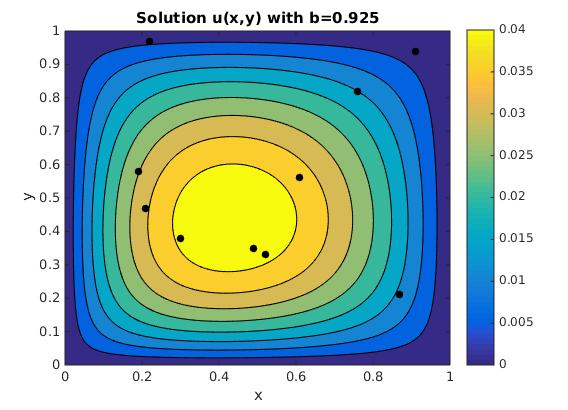
\includegraphics[scale=0.5]{./FigChap3/solu}
\caption{Numerical solution of the system (\ref{eqntoyproblem}) using a finite difference scheme. The mesh
size used in $x$ and $y$ was $0.01$. The value of the parameter $b$ was set at $0.925$. The black dots
in the plot represent the points used to generate the synthetic data about the experimental
measures $m$.}
\label{figsolU}
\end{figure}


At this point  we use the concept of emulator as in the previous chapter. If we had unlimited computational
power or time then we can run the finite difference scheme used to obtain Figure \ref{figsolU} with
a huge set of possible values for $b$ in the interval $(0,2]$. And pick the value that replicates the
better the syntetic data $m$. Since we do not have unlimited computational power or time what we
are going to do is to pick some $n$  values $b_{k}\in (0,2], k=1,2,\ldots,n$, run the finite difference
scheme on those and then use an emulator $\hat{f}$ with GPs to fill the missing data. The criteria to 
choose the number $n$ comes from considerations of how much time and computational resources we have.
For this case we chose $n=10$. How to distribute those 10 points in the interval $(0,2]$. Here we
use the concept space filling design. In the one dimensional setting it is not hard to see that
a maximin design gives an equal spacing of the 10 points in the interval $(0,2]$ hence we choose
\begin{equation*}
b_{k}=0.2k \qquad\text{for }k=1,2,\ldots,10.
\end{equation*}

We are ready to run the emulator $\hat{f}$ for these values of $b$, get a numerical value at
the 10 points in the domain where the synthetic data were created (black dots in Figure \ref{figsolU})
and use GPs to fill the missing information. Take into account that this process of `filling the blanks'
has to be done in all of the 10 measurement points in the domain $\Omega$ of definition of the phyiscal model.

In Figure \ref{fignofitted} we can see the results from running the emulator (black dots) compared
with the experimental measurement for each of the 10 sites (black line).

\begin{figure}[H]
\centering
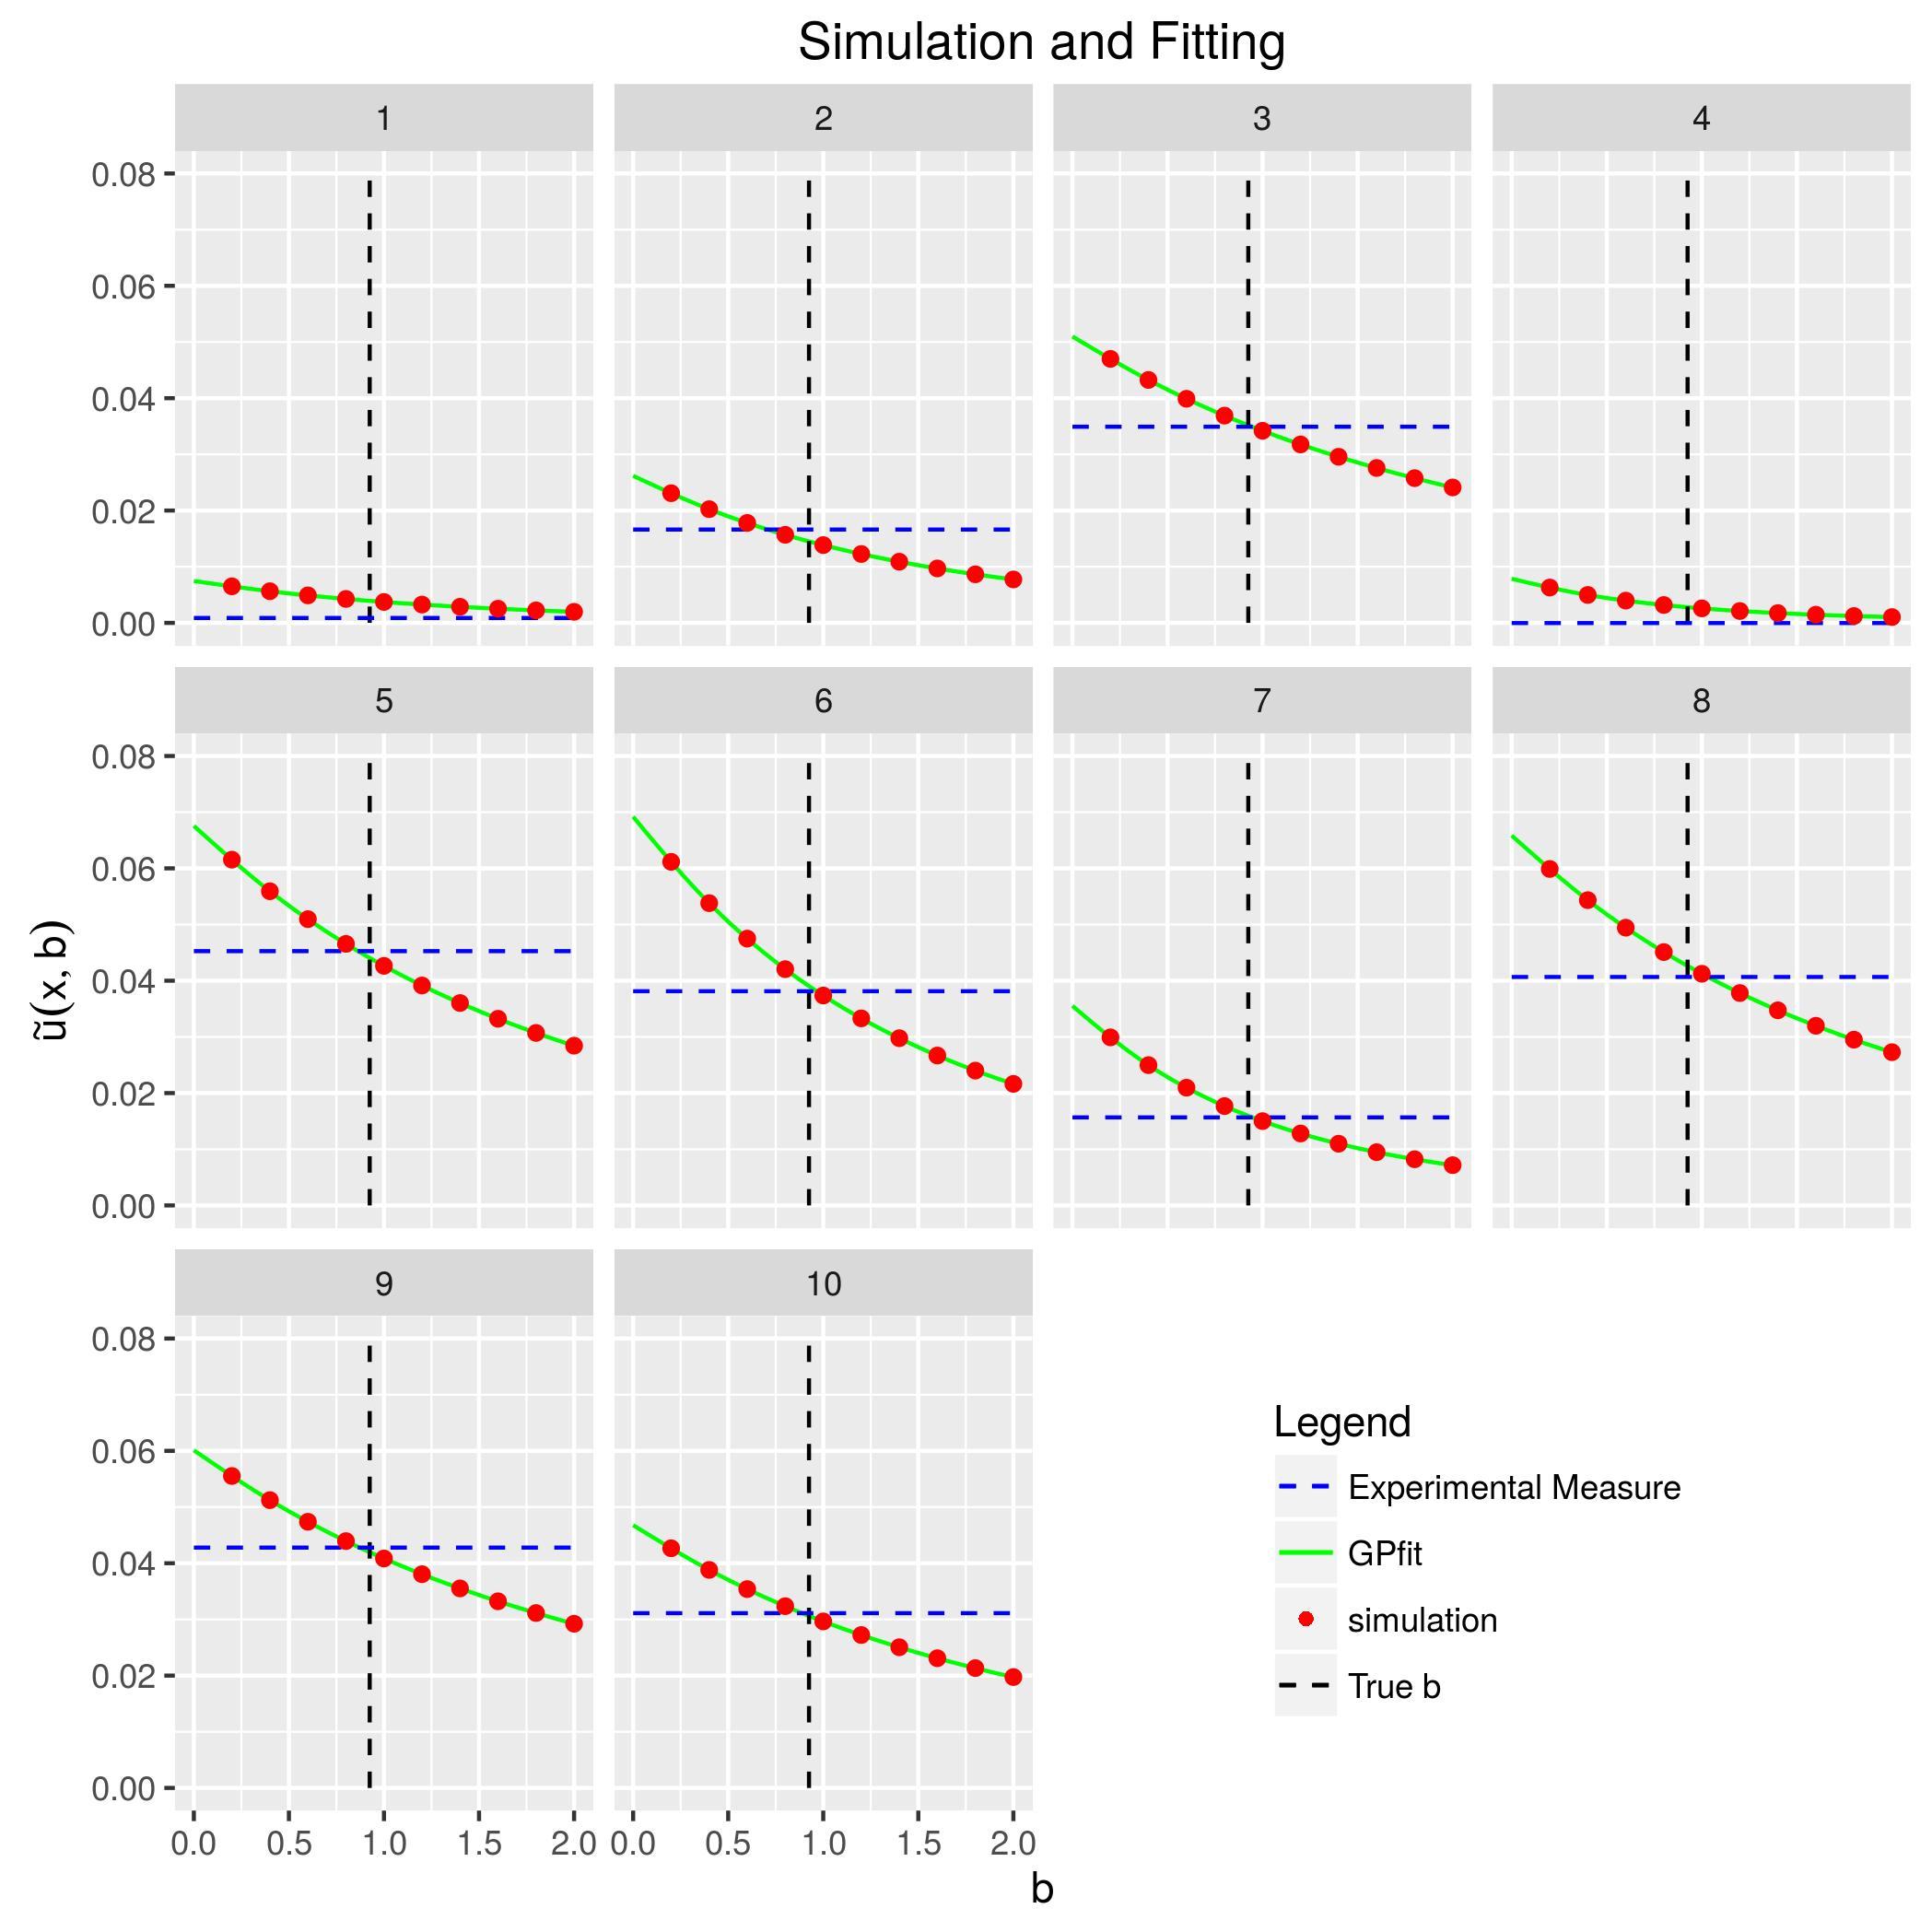
\includegraphics[scale=0.7]{./FigChap3/fitted}
\caption{whatever}
\label{fignofitted}
\end{figure}

As we can see in Figure \ref{fignofitted}, the emulator sometimes overestimates the value of $b$ and sometimes
underestimates it, this behaviour is expected. The hope is that this inaccuracies oscilate around the true
value of $b$.

Since we only have a limited number of prediction of the emulator for different values of $b$ (black points
in Figure \ref{fignofitted}), we would like to extrapolate/interpolate those results to get
more data and with that extra data, assess the value of $b$. As explained in Chapter 2, one very useful 
way to obtain the extra data is through Gaussian processes. Using the language of the previous chapter
what we want to do is, having the training points $\{(x_{i},f(x_{i})\}_{i=1}^{10}$ we want to predict 
the value of different test points $x_{i}^{*}$. This prediction is shown as a red line in Figure
\ref{fignofitted}.  The GP fit allows us to approxiamte as much value as we want, along with the uncertainty
associated with the prediction. Having this data we can now proceed to use the Bayesian methodology.
The idea goes as follows. if we denote the GP fit at at point $b$ as  $G(b)$, then we may assume
an additive noise model for the output $y$ as
\begin{equation}\label{eqnadditivenoise}
y=G(b)+\vec{\epsilon}.
\end{equation}
$\vec{\epsilon}$ is a random vector distributed as $\vec{\epsilon}\sim\mathscr{N}(0,\sigma I)$. Where $sigma=bla$
and $I$ is the $10\times 10$ identity matrix.
In the Bayesian framework we are interest in finding the value of $b$ given the experimental measurements $m$.
To that end we go back to the begining of this chapter and use equation (\ref{eqnpropto}). To use this equation
we need to find the likelihood $\like(m|b)$. Under the assumption of the additive noise model in equation
(\ref{eqnadditivenoise}) we get as in the smashed window example in chapter 2 that
\begin{equation*}
m|b\sim\mathscr{N}(G(b),\sigma I),
\end{equation*}
more precisely
\begin{equation*}
\like(m|b)=\frac{1}{(2\pi\sigma)^{n/2}}\exp\left(-\frac{\|G(b)-m\|_{2}^{2}}{2\sigma^{2}}\right).
\end{equation*}



Now we need to choose a prior for $b$. This is a delicate issue and a polemic one in the Statistics community.
The prior should reflect all of our current knowledge about $b$. However your knowledge about $b$ might be 
different than my knowledge about $b$, hence your prior for $b$ might look different than mine. For
the moment  we won't worry about that. Let's assume that our prior for $b$ is given by
\begin{equation*}
b\sim U(0,2).
\end{equation*}
where $U(a,b)$ is the uniform distribution in $a,b$. Putting all of this into formula (\ref{eqnpropto}) we get
\begin{equation*}
\post(b|m)\propto\chi_{[0,2]}\exp\left(-\frac{\|G(b)-m\|_{2}^{2}}{2\sigma^{2}}\right),
\end{equation*}
where $\chi_{[a,b]}$ is the indicator function of the set $[a,b]$. This equation can be 
interpreted as the update in knowledge from to prior to the posterior in the light of the
experimental data obtained represented by the likelihood. This change from prior to 
posterior is shown below.
\begin{figure}[H]
\centering
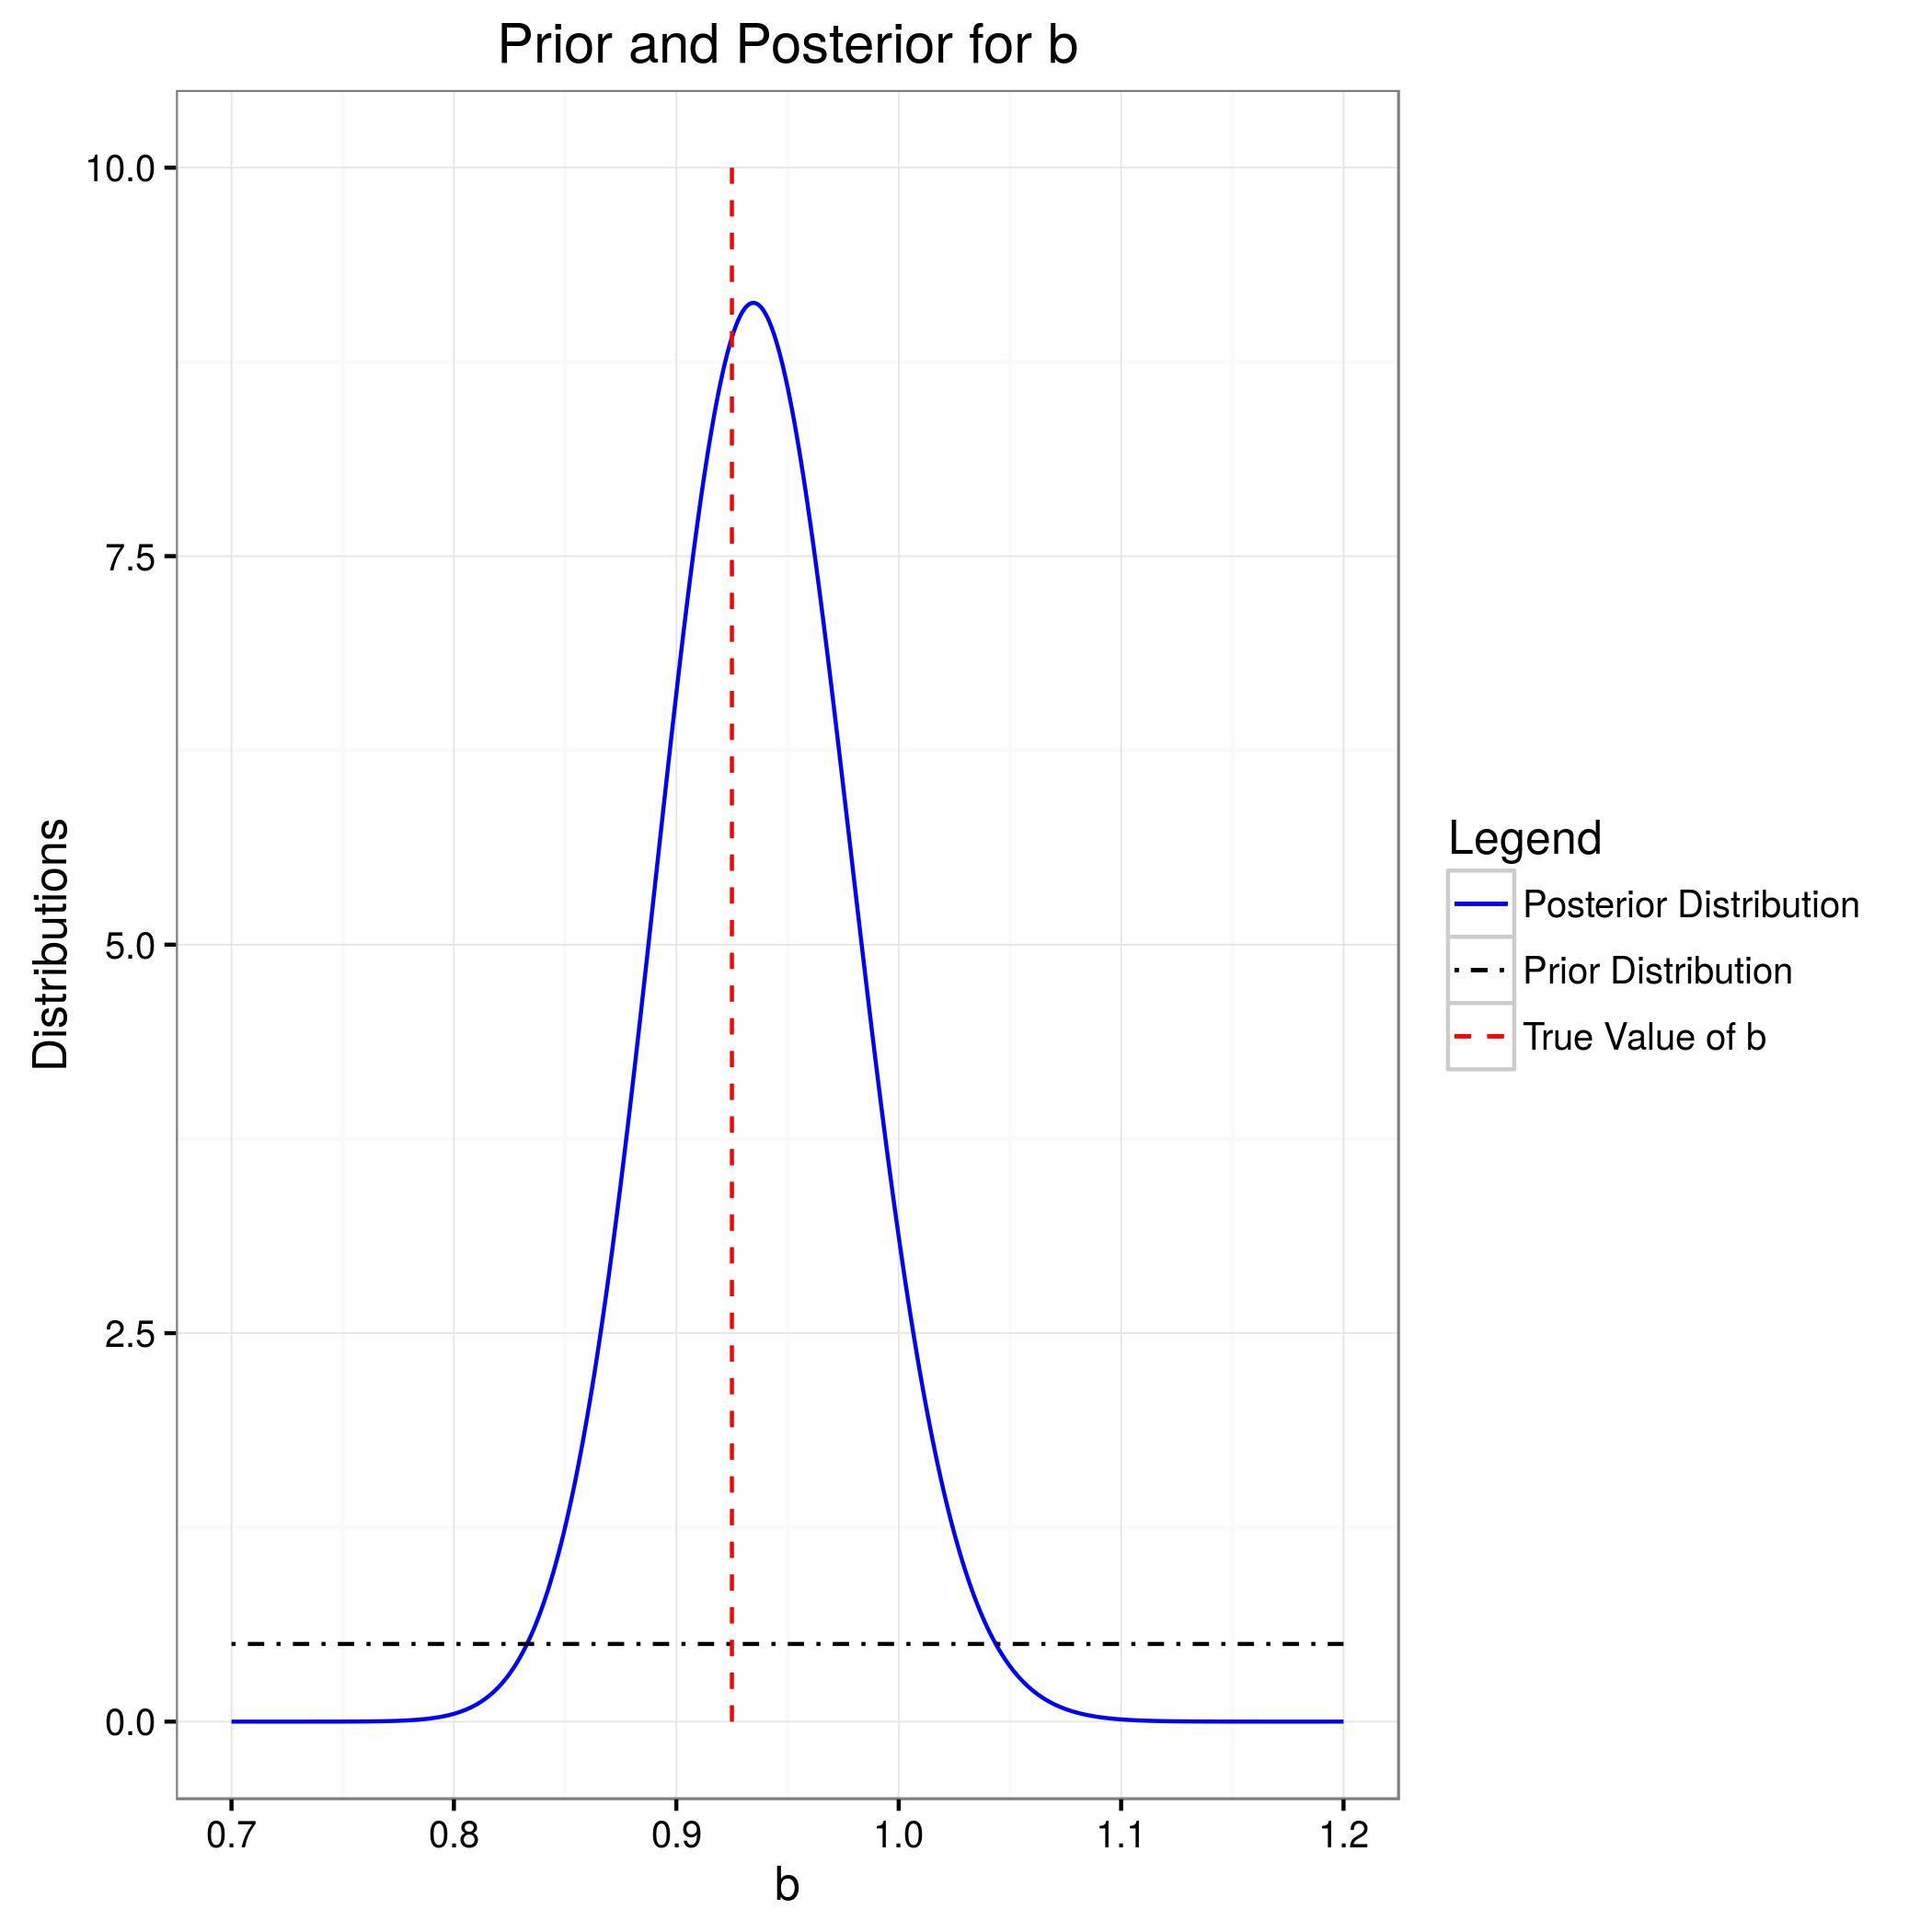
\includegraphics[scale=0.8]{./FigChap3/prior_posterior.jpg}
\caption{whatever}
\end{figure} 






As we mentioned in chapter 2,
the solution to an inverse problem in the Bayesian framework is the posterior. The question is:
how can we use this posterior to infer the value of $b$ and the uncertainty associated to it? 
\textbf{Here talk about how this integral is untractable}.

To make inferences about the value of $b$ we resort to a family of techniques from sampling probability
distributions known as Markov Chain Monte Carlo (MCMC)\textbf{Cite algun libro del MCMC}.

After using the MCMC we get the following plot 

\begin{figure}[H]
\centering
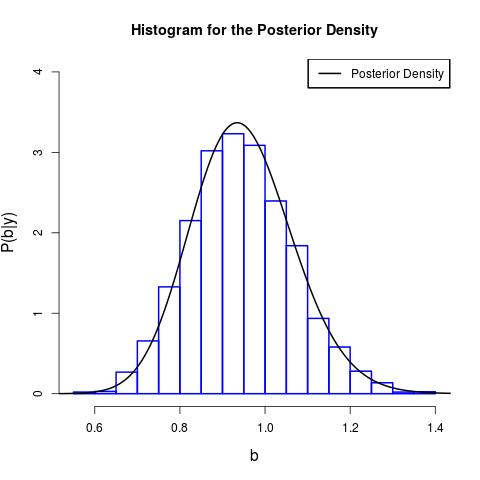
\includegraphics[scale=0.8]{./FigChap3/histogram_mcmc.jpg}
\caption{whatever}
\end{figure}



\subsection*{How important is the prior to make inferences?}
It is constructive to go in some depth and explore how prominent is the role of the prior probability
in making inferences about a problem. Let us consider the same problem as above, we want to estimate
the value of the paramter $b$. For demonstration purposes, let us assume two things. The parameter
$b$ can be any real number (not just $0<b\leq 2$ as before) and
\begin{equation*}
b\sim\mathscr{N}(b^{*},\sigma_{b}^{2}),
\end{equation*}
where $b^{*}$ and $\sigma_{b}$ are parameters to be set later.  With this new prior the formula
for the posterior becomes 
\begin{equation*}
\post(b|m)\propto \exp\left(-\frac{\|m-G(b)\|_{2}^{2}}{2\sigma^{2}}-\frac{(b-b^{*})^{2}}{2\sigma_{b}^{2}}\right).
\end{equation*}





As before, assume that the true
value of $b$ is $0.925$. To ilustrate the role that the prior has in the inference of the value
of $b$ given the experimental data $m$, let us assume that 
\begin{equation*}
b\sim\mathscr{N}(4,2.5).
\end{equation*}
That is, the person that proposed this prior is confident that within $95\%$ of confidence, the true value of
$b$ is in the interval $[1.8,8.2]$. Let us see what happens with the posterior in equation (\ref{eqnpropto})
when we get more and more experimental data. 
\begin{figure}[H]
\centering
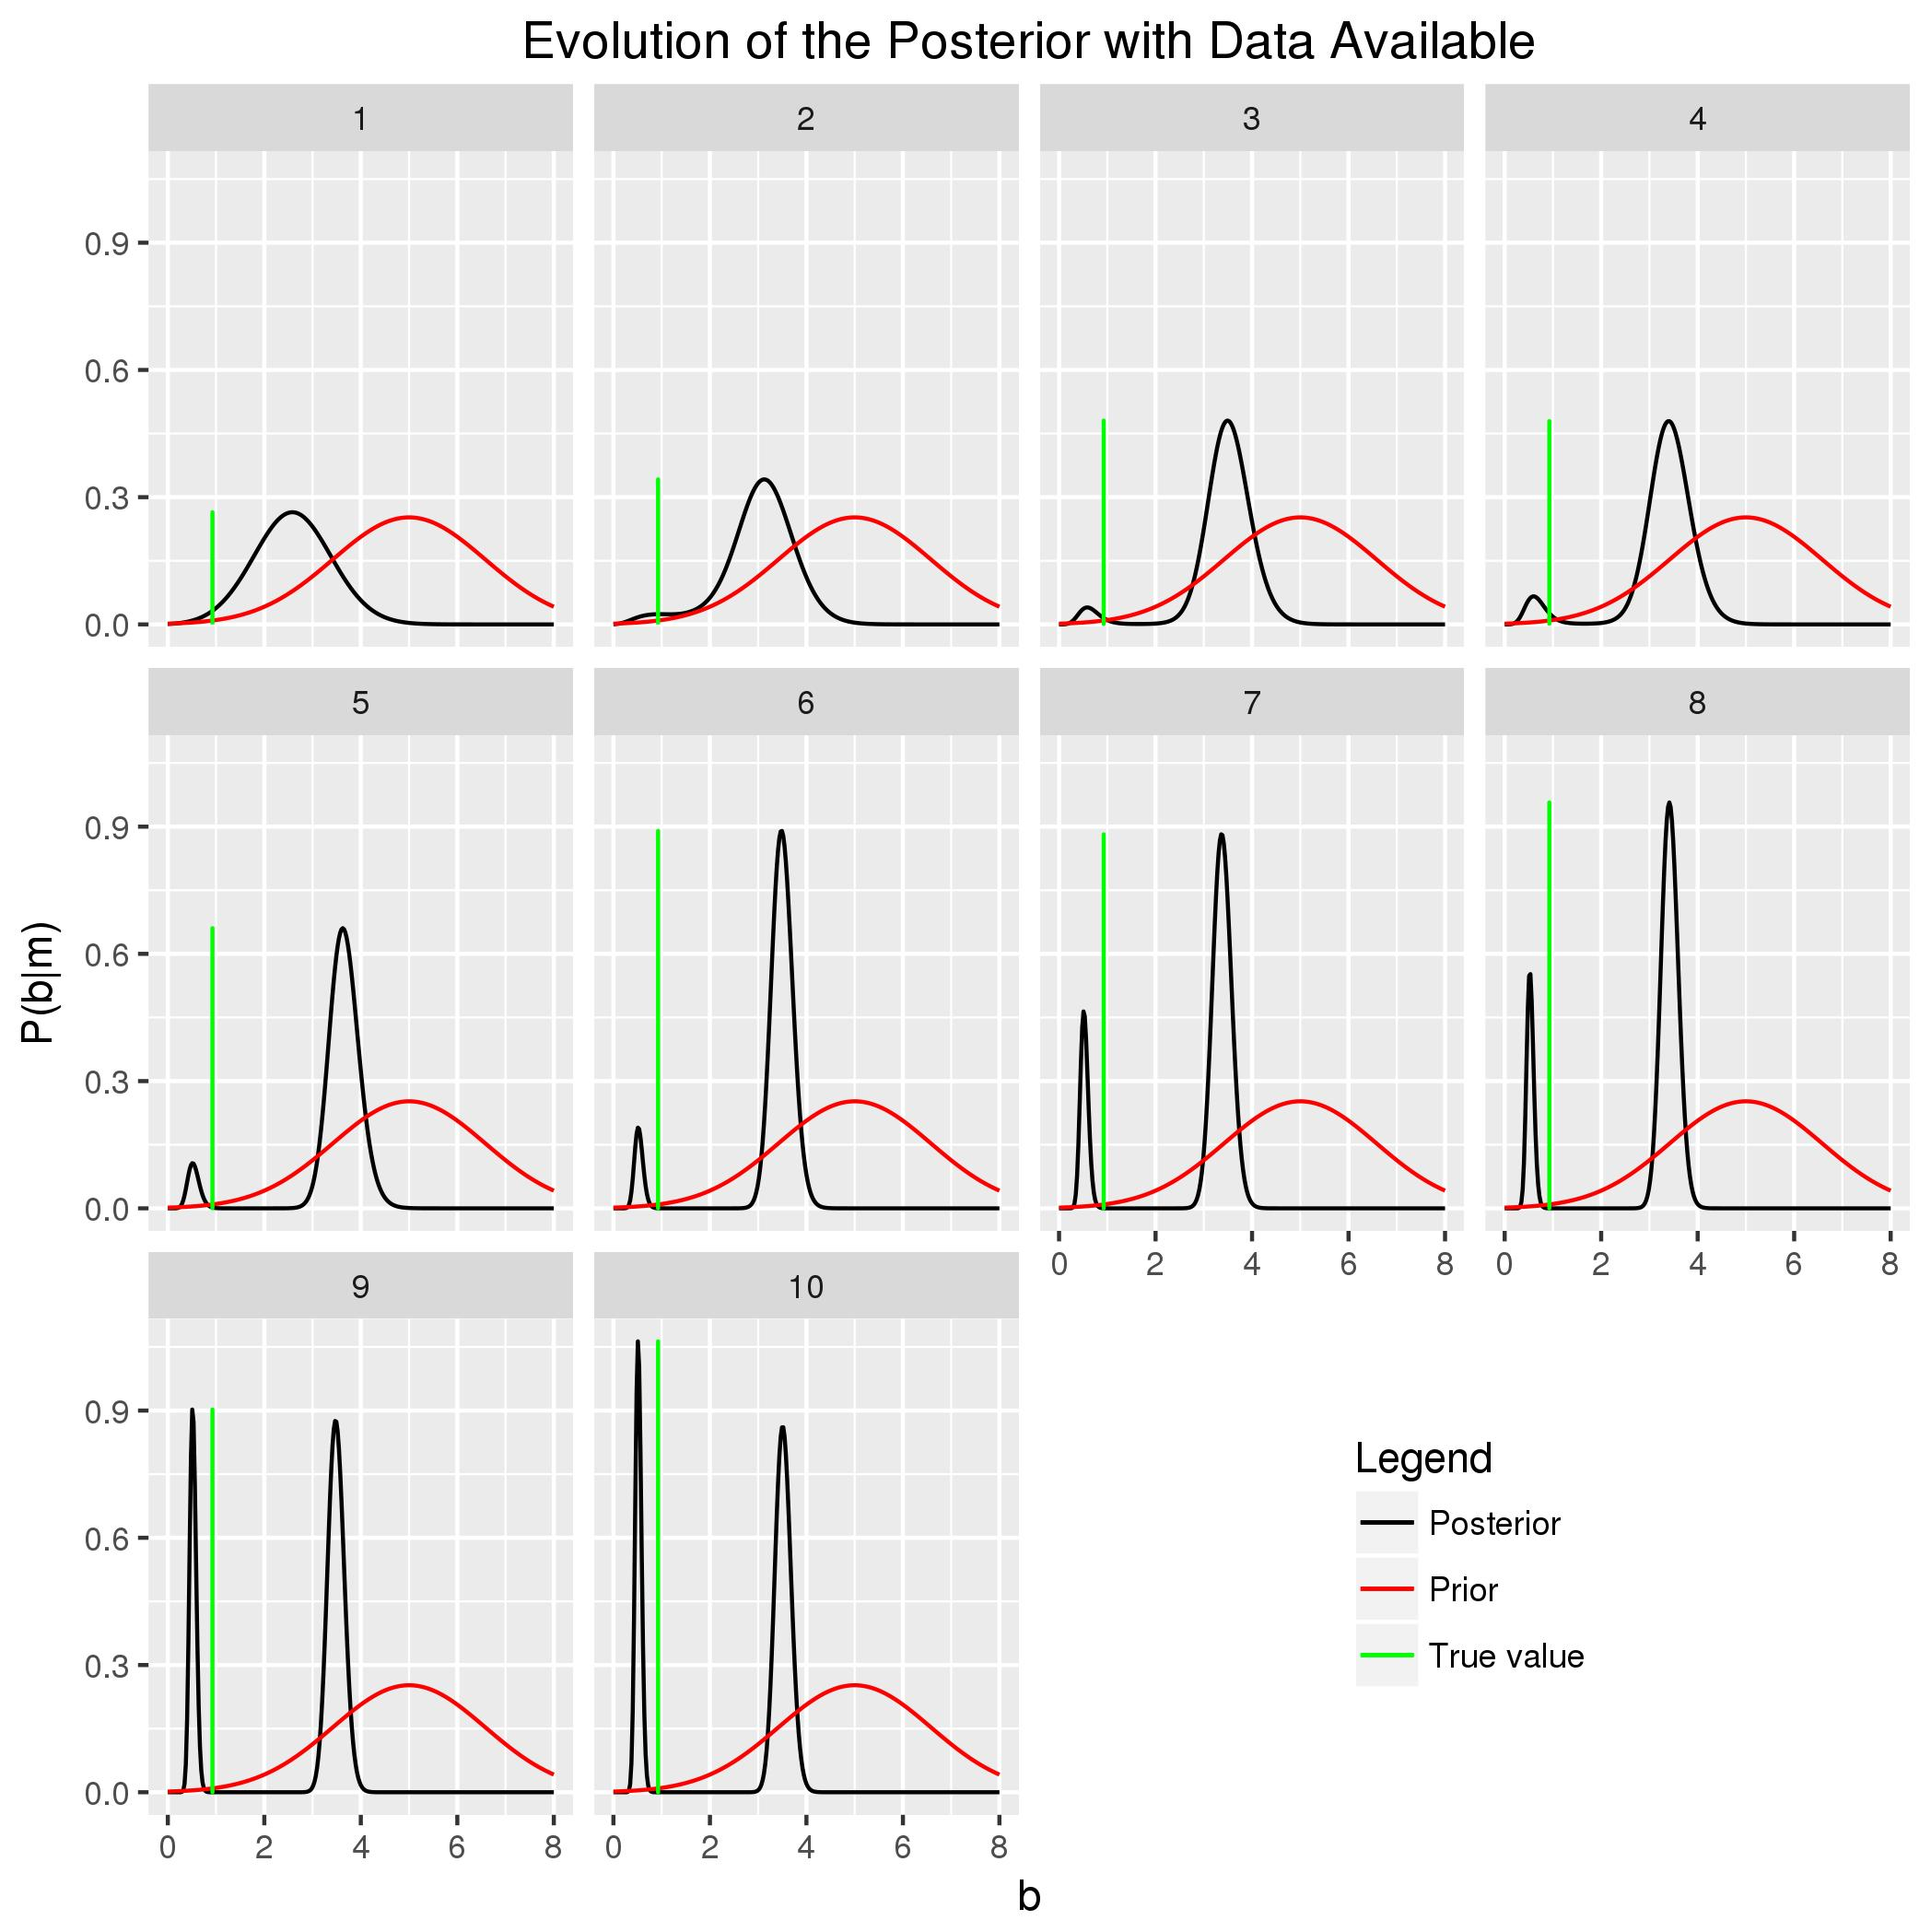
\includegraphics[scale=0.7]{./FigChap3/posterior_evolution}
\caption{bla}
\end{figure}
\bibliography{Tesis}
\bibliographystyle{plain}




\end{document}
